% =====================================================================
%  Informe de Simulación — IC al 95 % para p = 0.5
%  Versión: experimento MAS vs. determinista (n = 50, R = 10 000)
% =====================================================================
\documentclass[11pt,a4paper]{article}

% --------------------------- Paquetes --------------------------------
\usepackage[spanish]{babel}
\decimalpoint            % mantiene el punto decimal con babel antiguo
\usepackage[T1]{fontenc}
\usepackage[utf8]{inputenc}
\usepackage{geometry}
  \geometry{margin=2.5cm}
\usepackage{parskip}
\usepackage{setspace}\onehalfspacing
\usepackage{amsmath,amssymb}
\usepackage{booktabs,caption}
  \captionsetup{labelfont=bf,font=small,labelsep=period}
\usepackage{graphicx,float}
\usepackage[hidelinks]{hyperref}

% --------------------------- Datos -----------------------------------
\title{Efecto de la Falta de Aleatoriedad sobre la Cobertura de Intervalos de Confianza}
\author{Diego B. Meza Bogado}
\date{\today}

% =====================================================================
\begin{document}
\maketitle
\tableofcontents
\bigskip

% =====================================================================
\section{Diseño del experimento}
Se simulan $R=10\,000$ réplicas para una proporción poblacional $p=0.5$ bajo dos esquemas:
\begin{enumerate}
  \item \textbf{Muestreo aleatorio simple (MAS)}: cada réplica extrae $n=50$ observaciones i.i.d.~Bernoulli$(0.5)$.  
  \item \textbf{Muestra determinista}: los valores se generan mediante
        $y_i = \mathbf 1\{m\,i + b > 0\}$ con $m\sim\mathrm U(-0.05,0.05)$ y $b\sim\mathrm U(-2.5,2.5)$ sorteados por réplica, de modo que una vez fijados $(m,b)$ la muestra carece de variabilidad interna.
\end{enumerate}
Para cada muestra se estima $\hat p$ y se construye un IC de Wald al 95~\%
\[ IC_{95\%}=\hat p \pm 1.96\,\sqrt{\dfrac{\hat p(1-\hat p)}{n}}. \]

% =====================================================================
\section{Cobertura observada}
\begin{table}[H]
  \centering
  \caption{Proporción de IC que contienen el valor verdadero $p=0.5$ (R=10\,000).}
  \label{tab:cobertura}
  \begin{tabular}{@{}lc@{}}
    \toprule
    Diseño de muestreo & Cobertura \\
    \midrule
    Muestreo aleatorio simple (MAS) & 0.9336 \\
    Determinista (lineal)           & 0.0671 \\
    \bottomrule
  \end{tabular}
\end{table}
La cobertura bajo MAS se aproxima al 95~\% nominal, mientras que la muestra determinista apenas cubre el 6.7~\%, evidenciando la pérdida de validez al romper la aleatoriedad.

% =====================================================================
\section{Visualización de los IC}
La Figura~\ref{fig:intervalos} superpone los 10~000 intervalos de confianza de cada método. Las barras grises cubren $p=0.5$; las rojas no lo hacen.

\begin{figure}[H]
  \centering
  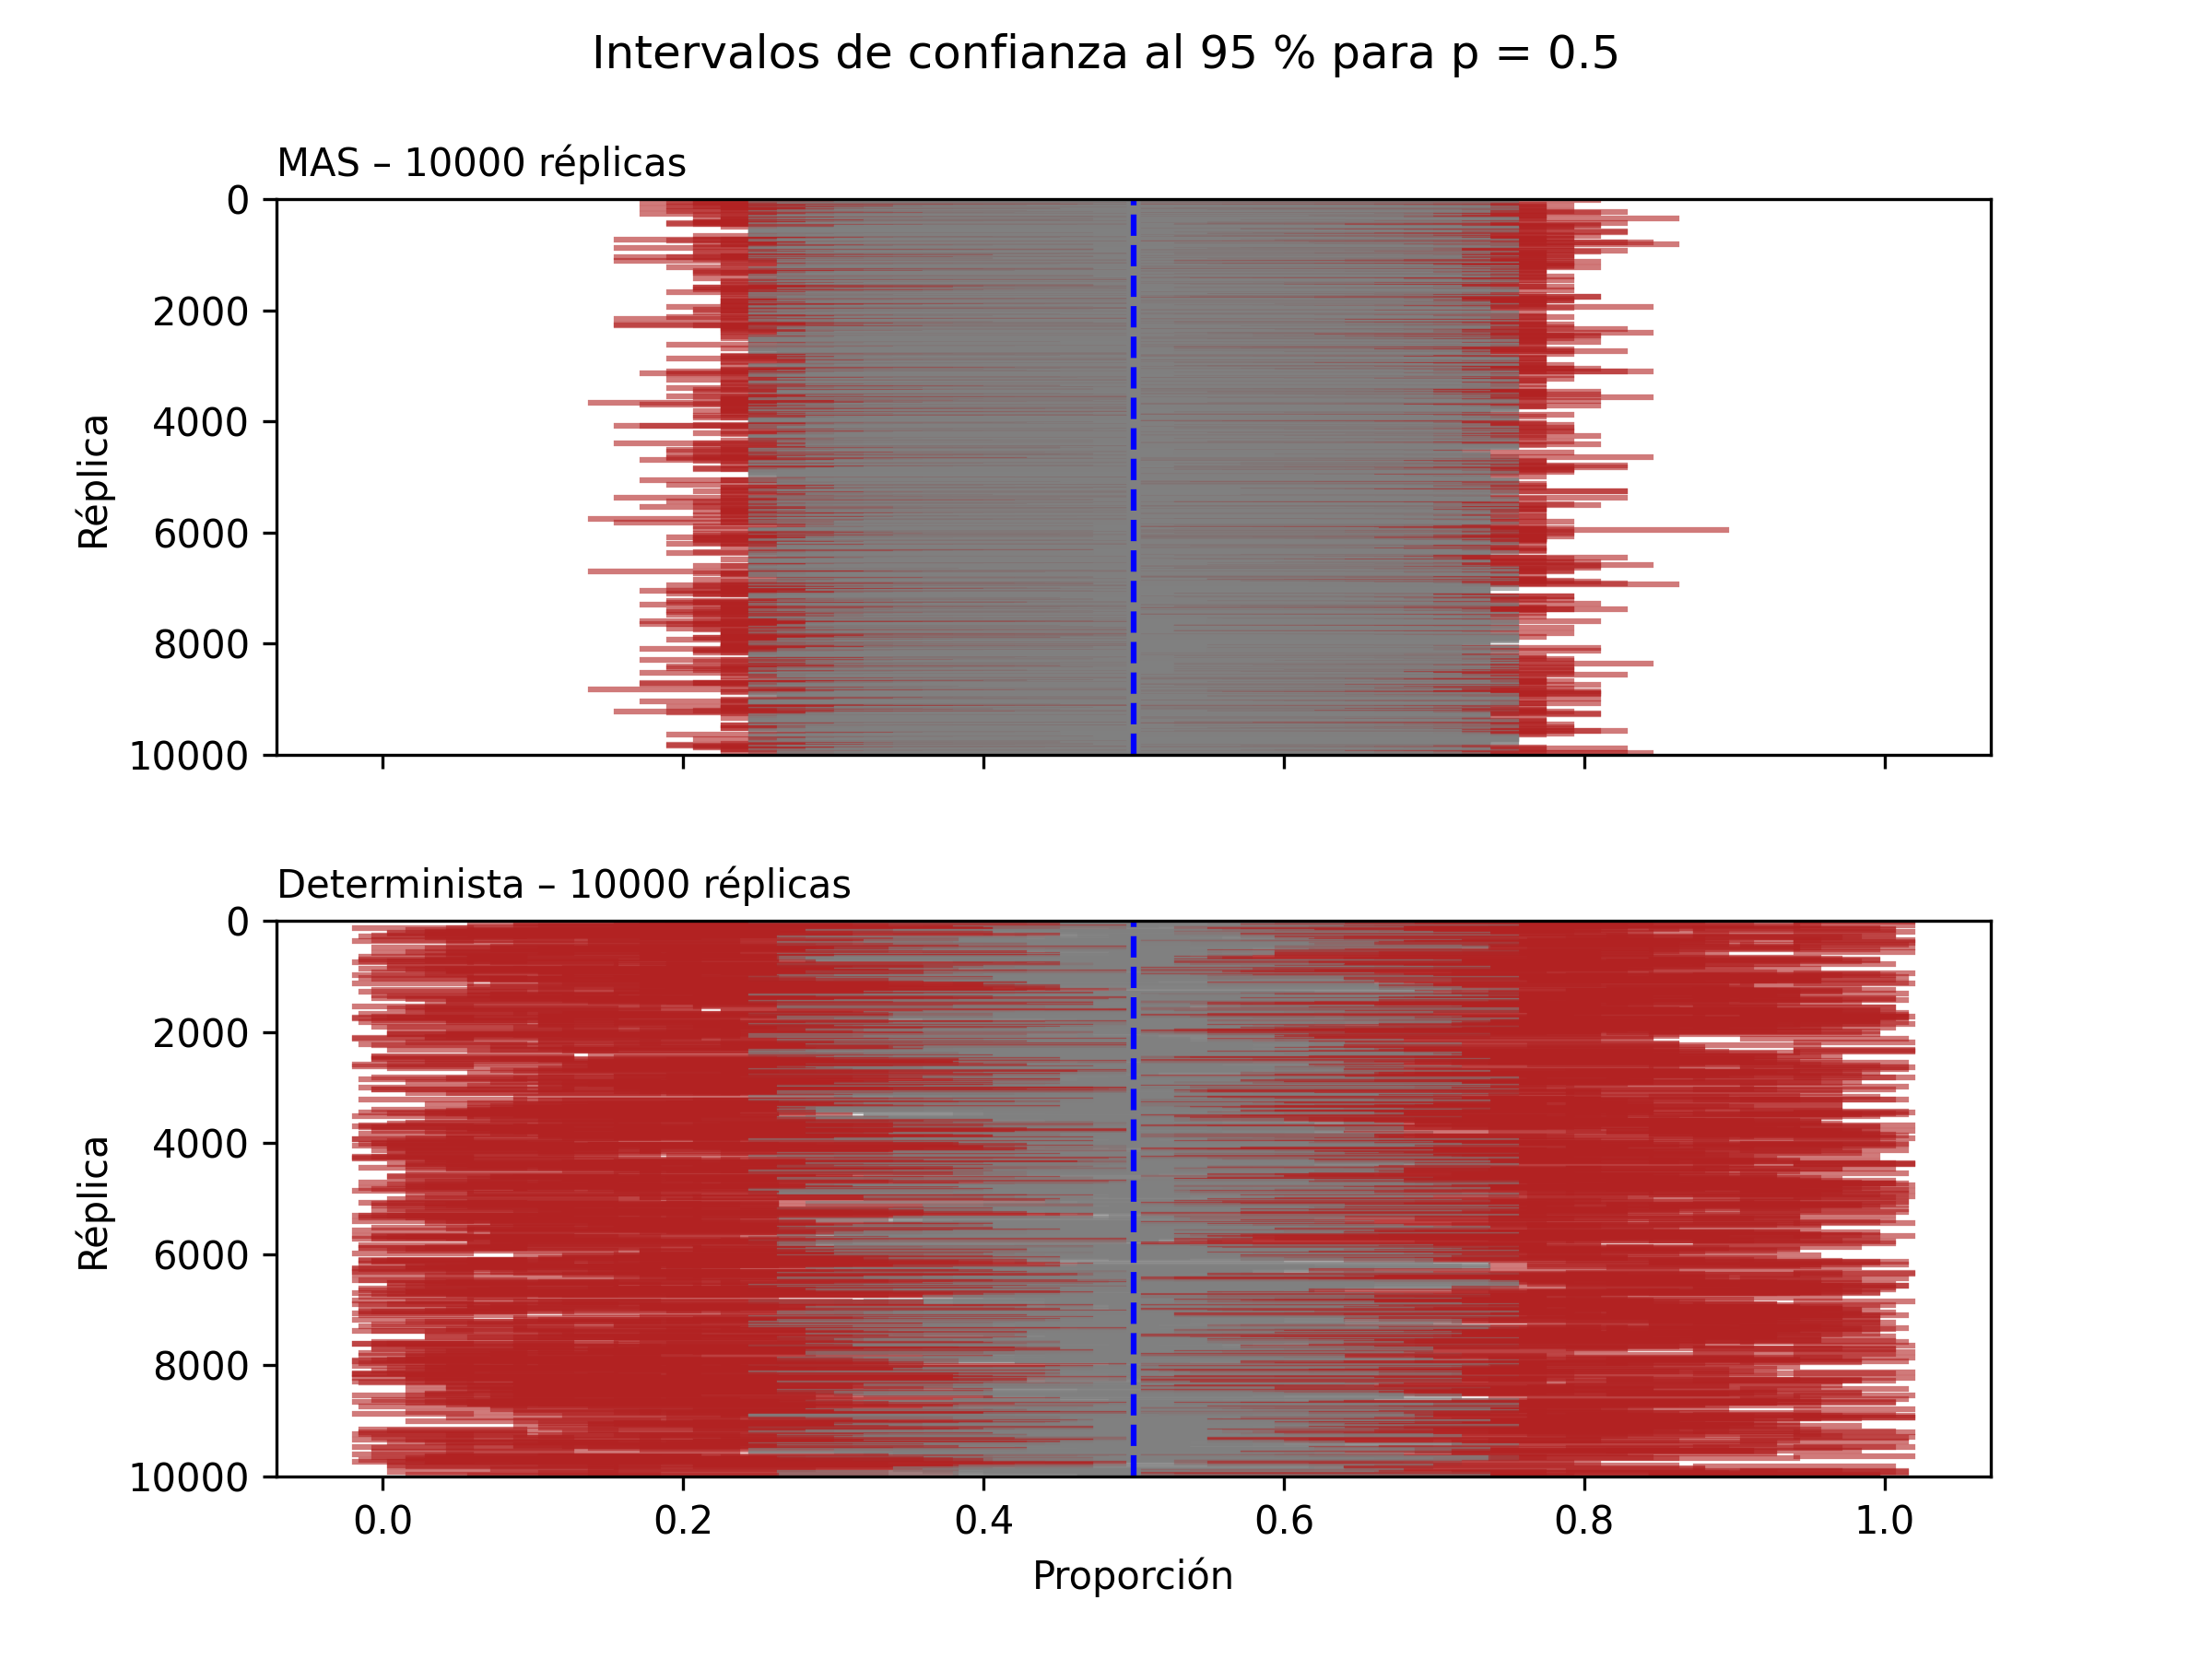
\includegraphics[width=0.9\textwidth]{intervalos_ic.png}
  \caption{Intervalos de confianza al 95~\% para $p=0.5$; comparación entre MAS y muestra determinista. La línea azul discontinua marca el valor verdadero.}
  \label{fig:intervalos}
\end{figure}

% =====================================================================
\section{Discusión}
El experimento demuestra que la fórmula clásica de Wald funciona cuando el supuesto de muestreo aleatorio se cumple; de lo contrario, el estimador $\hat p$ puede quedar sesgado y la varianza interna subestimar la incertidumbre real. Como resultado, los IC calculados en la muestra determinista son demasiado estrechos y rara vez incluyen $p=0.5$.

% =====================================================================
\section{Conclusiones}
\begin{itemize}
  \item El diseño de muestreo es determinante para la validez de los IC: sin aleatoriedad, la cobertura nominal queda anulada.
  \item Aumentar el tamaño muestral no corrige el sesgo de selección ni restaura la cobertura.  
  \item Estudios con muestras no probabilísticas deben aplicar ponderaciones o modelos de corrección para recuperar la inferencia.
\end{itemize}

\end{document}